% Graphic for TeX using PGF
% Title: /home/lnatale/Documents/xfire/digital/xfire_core/docs/thesis/tesis/figures/C02-global_predictor_2_2.dia
% Creator: Dia v0.97.3
% CreationDate: Mon Sep 12 14:51:44 2016
% For: lnatale
% \usepackage{tikz}
% The following commands are not supported in PSTricks at present
% We define them conditionally, so when they are implemented,
% this pgf file will use them.
\ifx\du\undefined
  \newlength{\du}
\fi
\setlength{\du}{15\unitlength}
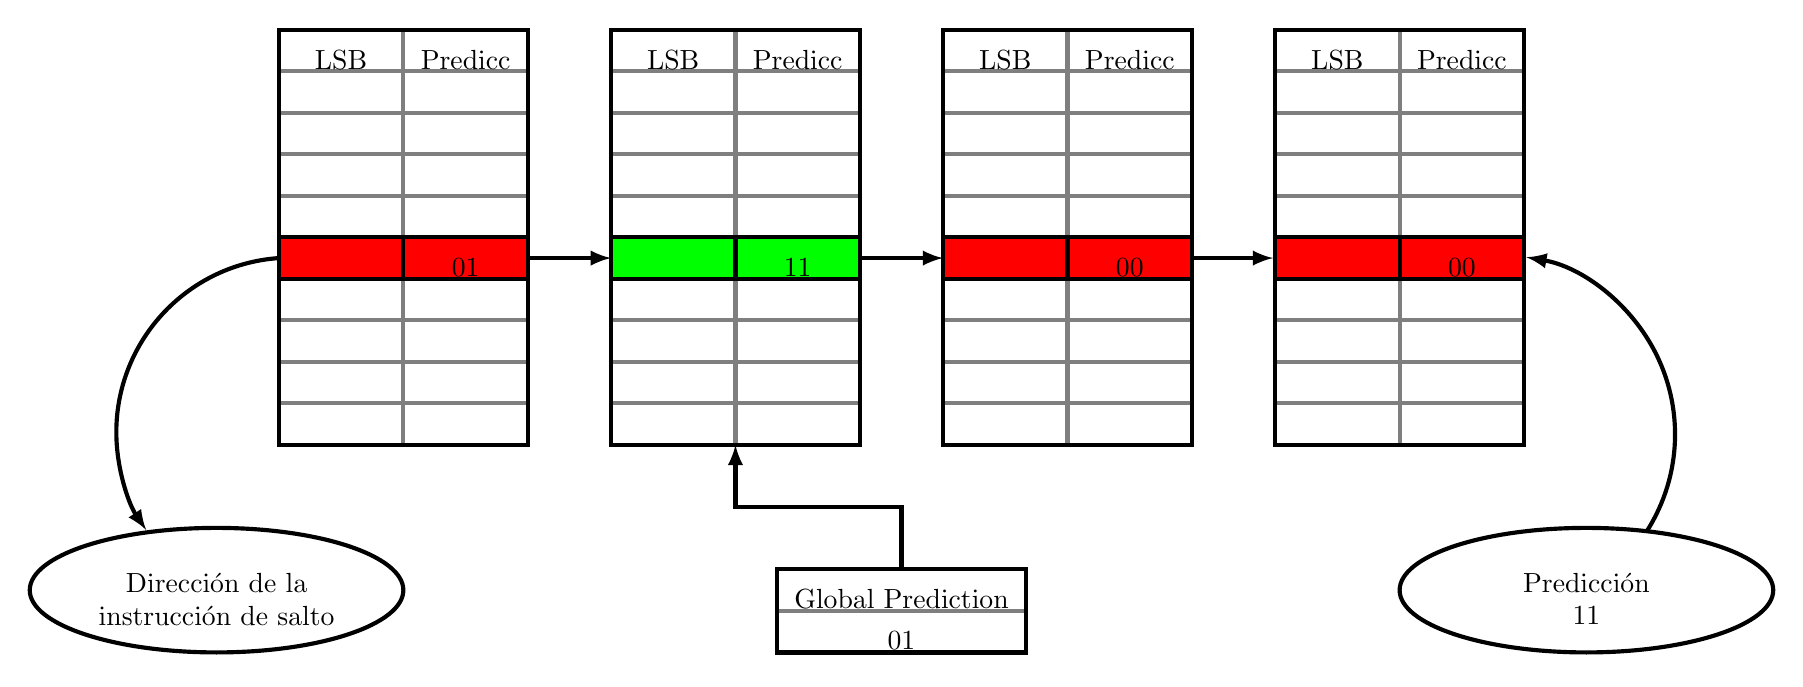
\begin{tikzpicture}
\pgftransformxscale{1.000000}
\pgftransformyscale{-1.000000}
\definecolor{dialinecolor}{rgb}{0.000000, 0.000000, 0.000000}
\pgfsetstrokecolor{dialinecolor}
\definecolor{dialinecolor}{rgb}{1.000000, 1.000000, 1.000000}
\pgfsetfillcolor{dialinecolor}
\pgfsetmiterjoin
\pgfsetdash{}{0pt}
\definecolor{dialinecolor}{rgb}{1.000000, 1.000000, 1.000000}
\pgfsetfillcolor{dialinecolor}
\fill (27.000000\du,20.000000\du)--(27.000000\du,22.000000\du)--(33.000000\du,22.000000\du)--(33.000000\du,20.000000\du)--cycle;
\pgfsetlinewidth{0.100000\du}
\definecolor{dialinecolor}{rgb}{0.498039, 0.498039, 0.498039}
\pgfsetstrokecolor{dialinecolor}
\draw (27.000000\du,21.000000\du)--(33.000000\du,21.000000\du);
\pgfsetlinewidth{0.100000\du}
\definecolor{dialinecolor}{rgb}{0.000000, 0.000000, 0.000000}
\pgfsetstrokecolor{dialinecolor}
\draw (27.000000\du,20.000000\du)--(27.000000\du,22.000000\du)--(33.000000\du,22.000000\du)--(33.000000\du,20.000000\du)--cycle;
\definecolor{dialinecolor}{rgb}{1.000000, 1.000000, 1.000000}
\pgfsetfillcolor{dialinecolor}
\pgfpathellipse{\pgfpoint{13.500000\du}{20.500000\du}}{\pgfpoint{4.500000\du}{0\du}}{\pgfpoint{0\du}{1.500000\du}}
\pgfusepath{fill}
\pgfsetlinewidth{0.100000\du}
\pgfsetdash{}{0pt}
\pgfsetdash{}{0pt}
\definecolor{dialinecolor}{rgb}{0.000000, 0.000000, 0.000000}
\pgfsetstrokecolor{dialinecolor}
\pgfpathellipse{\pgfpoint{13.500000\du}{20.500000\du}}{\pgfpoint{4.500000\du}{0\du}}{\pgfpoint{0\du}{1.500000\du}}
\pgfusepath{stroke}
% setfont left to latex
\definecolor{dialinecolor}{rgb}{0.000000, 0.000000, 0.000000}
\pgfsetstrokecolor{dialinecolor}
\node at (13.500000\du,20.322500\du){Dirección de la};
% setfont left to latex
\definecolor{dialinecolor}{rgb}{0.000000, 0.000000, 0.000000}
\pgfsetstrokecolor{dialinecolor}
\node at (13.500000\du,21.122500\du){instrucción de salto};
\pgfsetlinewidth{0.100000\du}
\pgfsetdash{}{0pt}
\pgfsetdash{}{0pt}
\pgfsetbuttcap
{
\definecolor{dialinecolor}{rgb}{0.000000, 0.000000, 0.000000}
\pgfsetfillcolor{dialinecolor}
% was here!!!
\pgfsetarrowsend{latex}
\definecolor{dialinecolor}{rgb}{0.000000, 0.000000, 0.000000}
\pgfsetstrokecolor{dialinecolor}
\pgfpathmoveto{\pgfpoint{15.000116\du}{12.499992\du}}
\pgfpatharc{266}{146}{4.208070\du and 4.208070\du}
\pgfusepath{stroke}
}
% setfont left to latex
\definecolor{dialinecolor}{rgb}{0.000000, 0.000000, 0.000000}
\pgfsetstrokecolor{dialinecolor}
\node at (30.000000\du,20.722500\du){Global Prediction};
% setfont left to latex
\definecolor{dialinecolor}{rgb}{0.000000, 0.000000, 0.000000}
\pgfsetstrokecolor{dialinecolor}
\node at (30.000000\du,21.722500\du){01};
\pgfsetlinewidth{0.100000\du}
\pgfsetdash{}{0pt}
\pgfsetdash{}{0pt}
\pgfsetmiterjoin
\pgfsetbuttcap
{
\definecolor{dialinecolor}{rgb}{0.000000, 0.000000, 0.000000}
\pgfsetfillcolor{dialinecolor}
% was here!!!
\pgfsetarrowsend{latex}
{\pgfsetcornersarced{\pgfpoint{0.000000\du}{0.000000\du}}\definecolor{dialinecolor}{rgb}{0.000000, 0.000000, 0.000000}
\pgfsetstrokecolor{dialinecolor}
\draw (30.000000\du,20.000000\du)--(30.000000\du,18.500000\du)--(26.000000\du,18.500000\du)--(26.000000\du,17.000000\du);
}}
\pgfsetmiterjoin
\pgfsetdash{}{0pt}
\definecolor{dialinecolor}{rgb}{1.000000, 1.000000, 1.000000}
\pgfsetfillcolor{dialinecolor}
\fill (39.000000\du,7.000000\du)--(39.000000\du,17.000000\du)--(45.000000\du,17.000000\du)--(45.000000\du,7.000000\du)--cycle;
\pgfsetlinewidth{0.100000\du}
\definecolor{dialinecolor}{rgb}{0.498039, 0.498039, 0.498039}
\pgfsetstrokecolor{dialinecolor}
\draw (39.000000\du,8.000000\du)--(45.000000\du,8.000000\du);
\definecolor{dialinecolor}{rgb}{0.498039, 0.498039, 0.498039}
\pgfsetstrokecolor{dialinecolor}
\draw (39.000000\du,9.000000\du)--(45.000000\du,9.000000\du);
\definecolor{dialinecolor}{rgb}{0.498039, 0.498039, 0.498039}
\pgfsetstrokecolor{dialinecolor}
\draw (39.000000\du,10.000000\du)--(45.000000\du,10.000000\du);
\definecolor{dialinecolor}{rgb}{0.498039, 0.498039, 0.498039}
\pgfsetstrokecolor{dialinecolor}
\draw (39.000000\du,11.000000\du)--(45.000000\du,11.000000\du);
\definecolor{dialinecolor}{rgb}{0.498039, 0.498039, 0.498039}
\pgfsetstrokecolor{dialinecolor}
\draw (39.000000\du,12.000000\du)--(45.000000\du,12.000000\du);
\definecolor{dialinecolor}{rgb}{0.498039, 0.498039, 0.498039}
\pgfsetstrokecolor{dialinecolor}
\draw (39.000000\du,13.000000\du)--(45.000000\du,13.000000\du);
\definecolor{dialinecolor}{rgb}{0.498039, 0.498039, 0.498039}
\pgfsetstrokecolor{dialinecolor}
\draw (39.000000\du,14.000000\du)--(45.000000\du,14.000000\du);
\definecolor{dialinecolor}{rgb}{0.498039, 0.498039, 0.498039}
\pgfsetstrokecolor{dialinecolor}
\draw (39.000000\du,15.000000\du)--(45.000000\du,15.000000\du);
\definecolor{dialinecolor}{rgb}{0.498039, 0.498039, 0.498039}
\pgfsetstrokecolor{dialinecolor}
\draw (39.000000\du,16.000000\du)--(45.000000\du,16.000000\du);
\definecolor{dialinecolor}{rgb}{0.498039, 0.498039, 0.498039}
\pgfsetstrokecolor{dialinecolor}
\draw (42.000000\du,7.000000\du)--(42.000000\du,17.000000\du);
\pgfsetlinewidth{0.100000\du}
\definecolor{dialinecolor}{rgb}{0.000000, 0.000000, 0.000000}
\pgfsetstrokecolor{dialinecolor}
\draw (39.000000\du,7.000000\du)--(39.000000\du,17.000000\du)--(45.000000\du,17.000000\du)--(45.000000\du,7.000000\du)--cycle;
% setfont left to latex
\definecolor{dialinecolor}{rgb}{0.000000, 0.000000, 0.000000}
\pgfsetstrokecolor{dialinecolor}
\node at (40.500000\du,7.722500\du){LSB};
% setfont left to latex
\definecolor{dialinecolor}{rgb}{0.000000, 0.000000, 0.000000}
\pgfsetstrokecolor{dialinecolor}
\node at (43.500000\du,7.722500\du){Predicc};
\pgfsetlinewidth{0.100000\du}
\pgfsetdash{}{0pt}
\pgfsetdash{}{0pt}
\pgfsetmiterjoin
\definecolor{dialinecolor}{rgb}{1.000000, 0.000000, 0.000000}
\pgfsetfillcolor{dialinecolor}
\fill (39.000000\du,12.000000\du)--(39.000000\du,13.000000\du)--(42.000000\du,13.000000\du)--(42.000000\du,12.000000\du)--cycle;
\definecolor{dialinecolor}{rgb}{0.000000, 0.000000, 0.000000}
\pgfsetstrokecolor{dialinecolor}
\draw (39.000000\du,12.000000\du)--(39.000000\du,13.000000\du)--(42.000000\du,13.000000\du)--(42.000000\du,12.000000\du)--cycle;
\pgfsetlinewidth{0.100000\du}
\pgfsetdash{}{0pt}
\pgfsetdash{}{0pt}
\pgfsetmiterjoin
\definecolor{dialinecolor}{rgb}{1.000000, 0.000000, 0.000000}
\pgfsetfillcolor{dialinecolor}
\fill (42.000000\du,12.000000\du)--(42.000000\du,13.000000\du)--(45.000000\du,13.000000\du)--(45.000000\du,12.000000\du)--cycle;
\definecolor{dialinecolor}{rgb}{0.000000, 0.000000, 0.000000}
\pgfsetstrokecolor{dialinecolor}
\draw (42.000000\du,12.000000\du)--(42.000000\du,13.000000\du)--(45.000000\du,13.000000\du)--(45.000000\du,12.000000\du)--cycle;
% setfont left to latex
\definecolor{dialinecolor}{rgb}{0.000000, 0.000000, 0.000000}
\pgfsetstrokecolor{dialinecolor}
\node at (43.500000\du,12.722500\du){00};
\pgfsetmiterjoin
\pgfsetdash{}{0pt}
\definecolor{dialinecolor}{rgb}{1.000000, 1.000000, 1.000000}
\pgfsetfillcolor{dialinecolor}
\fill (31.000000\du,7.000000\du)--(31.000000\du,17.000000\du)--(37.000000\du,17.000000\du)--(37.000000\du,7.000000\du)--cycle;
\pgfsetlinewidth{0.100000\du}
\definecolor{dialinecolor}{rgb}{0.498039, 0.498039, 0.498039}
\pgfsetstrokecolor{dialinecolor}
\draw (31.000000\du,8.000000\du)--(37.000000\du,8.000000\du);
\definecolor{dialinecolor}{rgb}{0.498039, 0.498039, 0.498039}
\pgfsetstrokecolor{dialinecolor}
\draw (31.000000\du,9.000000\du)--(37.000000\du,9.000000\du);
\definecolor{dialinecolor}{rgb}{0.498039, 0.498039, 0.498039}
\pgfsetstrokecolor{dialinecolor}
\draw (31.000000\du,10.000000\du)--(37.000000\du,10.000000\du);
\definecolor{dialinecolor}{rgb}{0.498039, 0.498039, 0.498039}
\pgfsetstrokecolor{dialinecolor}
\draw (31.000000\du,11.000000\du)--(37.000000\du,11.000000\du);
\definecolor{dialinecolor}{rgb}{0.498039, 0.498039, 0.498039}
\pgfsetstrokecolor{dialinecolor}
\draw (31.000000\du,12.000000\du)--(37.000000\du,12.000000\du);
\definecolor{dialinecolor}{rgb}{0.498039, 0.498039, 0.498039}
\pgfsetstrokecolor{dialinecolor}
\draw (31.000000\du,13.000000\du)--(37.000000\du,13.000000\du);
\definecolor{dialinecolor}{rgb}{0.498039, 0.498039, 0.498039}
\pgfsetstrokecolor{dialinecolor}
\draw (31.000000\du,14.000000\du)--(37.000000\du,14.000000\du);
\definecolor{dialinecolor}{rgb}{0.498039, 0.498039, 0.498039}
\pgfsetstrokecolor{dialinecolor}
\draw (31.000000\du,15.000000\du)--(37.000000\du,15.000000\du);
\definecolor{dialinecolor}{rgb}{0.498039, 0.498039, 0.498039}
\pgfsetstrokecolor{dialinecolor}
\draw (31.000000\du,16.000000\du)--(37.000000\du,16.000000\du);
\definecolor{dialinecolor}{rgb}{0.498039, 0.498039, 0.498039}
\pgfsetstrokecolor{dialinecolor}
\draw (34.000000\du,7.000000\du)--(34.000000\du,17.000000\du);
\pgfsetlinewidth{0.100000\du}
\definecolor{dialinecolor}{rgb}{0.000000, 0.000000, 0.000000}
\pgfsetstrokecolor{dialinecolor}
\draw (31.000000\du,7.000000\du)--(31.000000\du,17.000000\du)--(37.000000\du,17.000000\du)--(37.000000\du,7.000000\du)--cycle;
% setfont left to latex
\definecolor{dialinecolor}{rgb}{0.000000, 0.000000, 0.000000}
\pgfsetstrokecolor{dialinecolor}
\node at (32.500000\du,7.722500\du){LSB};
% setfont left to latex
\definecolor{dialinecolor}{rgb}{0.000000, 0.000000, 0.000000}
\pgfsetstrokecolor{dialinecolor}
\node at (35.500000\du,7.722500\du){Predicc};
\pgfsetlinewidth{0.100000\du}
\pgfsetdash{}{0pt}
\pgfsetdash{}{0pt}
\pgfsetmiterjoin
\definecolor{dialinecolor}{rgb}{1.000000, 0.000000, 0.000000}
\pgfsetfillcolor{dialinecolor}
\fill (31.000000\du,12.000000\du)--(31.000000\du,13.000000\du)--(34.000000\du,13.000000\du)--(34.000000\du,12.000000\du)--cycle;
\definecolor{dialinecolor}{rgb}{0.000000, 0.000000, 0.000000}
\pgfsetstrokecolor{dialinecolor}
\draw (31.000000\du,12.000000\du)--(31.000000\du,13.000000\du)--(34.000000\du,13.000000\du)--(34.000000\du,12.000000\du)--cycle;
\pgfsetlinewidth{0.100000\du}
\pgfsetdash{}{0pt}
\pgfsetdash{}{0pt}
\pgfsetmiterjoin
\definecolor{dialinecolor}{rgb}{1.000000, 0.000000, 0.000000}
\pgfsetfillcolor{dialinecolor}
\fill (34.000000\du,12.000000\du)--(34.000000\du,13.000000\du)--(37.000000\du,13.000000\du)--(37.000000\du,12.000000\du)--cycle;
\definecolor{dialinecolor}{rgb}{0.000000, 0.000000, 0.000000}
\pgfsetstrokecolor{dialinecolor}
\draw (34.000000\du,12.000000\du)--(34.000000\du,13.000000\du)--(37.000000\du,13.000000\du)--(37.000000\du,12.000000\du)--cycle;
% setfont left to latex
\definecolor{dialinecolor}{rgb}{0.000000, 0.000000, 0.000000}
\pgfsetstrokecolor{dialinecolor}
\node at (35.500000\du,12.722500\du){00};
\pgfsetmiterjoin
\pgfsetdash{}{0pt}
\definecolor{dialinecolor}{rgb}{1.000000, 1.000000, 1.000000}
\pgfsetfillcolor{dialinecolor}
\fill (23.000000\du,7.000000\du)--(23.000000\du,17.000000\du)--(29.000000\du,17.000000\du)--(29.000000\du,7.000000\du)--cycle;
\pgfsetlinewidth{0.100000\du}
\definecolor{dialinecolor}{rgb}{0.498039, 0.498039, 0.498039}
\pgfsetstrokecolor{dialinecolor}
\draw (23.000000\du,8.000000\du)--(29.000000\du,8.000000\du);
\definecolor{dialinecolor}{rgb}{0.498039, 0.498039, 0.498039}
\pgfsetstrokecolor{dialinecolor}
\draw (23.000000\du,9.000000\du)--(29.000000\du,9.000000\du);
\definecolor{dialinecolor}{rgb}{0.498039, 0.498039, 0.498039}
\pgfsetstrokecolor{dialinecolor}
\draw (23.000000\du,10.000000\du)--(29.000000\du,10.000000\du);
\definecolor{dialinecolor}{rgb}{0.498039, 0.498039, 0.498039}
\pgfsetstrokecolor{dialinecolor}
\draw (23.000000\du,11.000000\du)--(29.000000\du,11.000000\du);
\definecolor{dialinecolor}{rgb}{0.498039, 0.498039, 0.498039}
\pgfsetstrokecolor{dialinecolor}
\draw (23.000000\du,12.000000\du)--(29.000000\du,12.000000\du);
\definecolor{dialinecolor}{rgb}{0.498039, 0.498039, 0.498039}
\pgfsetstrokecolor{dialinecolor}
\draw (23.000000\du,13.000000\du)--(29.000000\du,13.000000\du);
\definecolor{dialinecolor}{rgb}{0.498039, 0.498039, 0.498039}
\pgfsetstrokecolor{dialinecolor}
\draw (23.000000\du,14.000000\du)--(29.000000\du,14.000000\du);
\definecolor{dialinecolor}{rgb}{0.498039, 0.498039, 0.498039}
\pgfsetstrokecolor{dialinecolor}
\draw (23.000000\du,15.000000\du)--(29.000000\du,15.000000\du);
\definecolor{dialinecolor}{rgb}{0.498039, 0.498039, 0.498039}
\pgfsetstrokecolor{dialinecolor}
\draw (23.000000\du,16.000000\du)--(29.000000\du,16.000000\du);
\definecolor{dialinecolor}{rgb}{0.498039, 0.498039, 0.498039}
\pgfsetstrokecolor{dialinecolor}
\draw (26.000000\du,7.000000\du)--(26.000000\du,17.000000\du);
\pgfsetlinewidth{0.100000\du}
\definecolor{dialinecolor}{rgb}{0.000000, 0.000000, 0.000000}
\pgfsetstrokecolor{dialinecolor}
\draw (23.000000\du,7.000000\du)--(23.000000\du,17.000000\du)--(29.000000\du,17.000000\du)--(29.000000\du,7.000000\du)--cycle;
% setfont left to latex
\definecolor{dialinecolor}{rgb}{0.000000, 0.000000, 0.000000}
\pgfsetstrokecolor{dialinecolor}
\node at (24.500000\du,7.722500\du){LSB};
% setfont left to latex
\definecolor{dialinecolor}{rgb}{0.000000, 0.000000, 0.000000}
\pgfsetstrokecolor{dialinecolor}
\node at (27.500000\du,7.722500\du){Predicc};
\pgfsetlinewidth{0.100000\du}
\pgfsetdash{}{0pt}
\pgfsetdash{}{0pt}
\pgfsetmiterjoin
\definecolor{dialinecolor}{rgb}{0.000000, 1.000000, 0.000000}
\pgfsetfillcolor{dialinecolor}
\fill (23.000000\du,12.000000\du)--(23.000000\du,13.000000\du)--(26.000000\du,13.000000\du)--(26.000000\du,12.000000\du)--cycle;
\definecolor{dialinecolor}{rgb}{0.000000, 0.000000, 0.000000}
\pgfsetstrokecolor{dialinecolor}
\draw (23.000000\du,12.000000\du)--(23.000000\du,13.000000\du)--(26.000000\du,13.000000\du)--(26.000000\du,12.000000\du)--cycle;
\pgfsetlinewidth{0.100000\du}
\pgfsetdash{}{0pt}
\pgfsetdash{}{0pt}
\pgfsetmiterjoin
\definecolor{dialinecolor}{rgb}{0.000000, 1.000000, 0.000000}
\pgfsetfillcolor{dialinecolor}
\fill (26.000000\du,12.000000\du)--(26.000000\du,13.000000\du)--(29.000000\du,13.000000\du)--(29.000000\du,12.000000\du)--cycle;
\definecolor{dialinecolor}{rgb}{0.000000, 0.000000, 0.000000}
\pgfsetstrokecolor{dialinecolor}
\draw (26.000000\du,12.000000\du)--(26.000000\du,13.000000\du)--(29.000000\du,13.000000\du)--(29.000000\du,12.000000\du)--cycle;
% setfont left to latex
\definecolor{dialinecolor}{rgb}{0.000000, 0.000000, 0.000000}
\pgfsetstrokecolor{dialinecolor}
\node at (27.500000\du,12.722500\du){11};
\pgfsetmiterjoin
\pgfsetdash{}{0pt}
\definecolor{dialinecolor}{rgb}{1.000000, 1.000000, 1.000000}
\pgfsetfillcolor{dialinecolor}
\fill (15.000000\du,7.000000\du)--(15.000000\du,17.000000\du)--(21.000000\du,17.000000\du)--(21.000000\du,7.000000\du)--cycle;
\pgfsetlinewidth{0.100000\du}
\definecolor{dialinecolor}{rgb}{0.498039, 0.498039, 0.498039}
\pgfsetstrokecolor{dialinecolor}
\draw (15.000000\du,8.000000\du)--(21.000000\du,8.000000\du);
\definecolor{dialinecolor}{rgb}{0.498039, 0.498039, 0.498039}
\pgfsetstrokecolor{dialinecolor}
\draw (15.000000\du,9.000000\du)--(21.000000\du,9.000000\du);
\definecolor{dialinecolor}{rgb}{0.498039, 0.498039, 0.498039}
\pgfsetstrokecolor{dialinecolor}
\draw (15.000000\du,10.000000\du)--(21.000000\du,10.000000\du);
\definecolor{dialinecolor}{rgb}{0.498039, 0.498039, 0.498039}
\pgfsetstrokecolor{dialinecolor}
\draw (15.000000\du,11.000000\du)--(21.000000\du,11.000000\du);
\definecolor{dialinecolor}{rgb}{0.498039, 0.498039, 0.498039}
\pgfsetstrokecolor{dialinecolor}
\draw (15.000000\du,12.000000\du)--(21.000000\du,12.000000\du);
\definecolor{dialinecolor}{rgb}{0.498039, 0.498039, 0.498039}
\pgfsetstrokecolor{dialinecolor}
\draw (15.000000\du,13.000000\du)--(21.000000\du,13.000000\du);
\definecolor{dialinecolor}{rgb}{0.498039, 0.498039, 0.498039}
\pgfsetstrokecolor{dialinecolor}
\draw (15.000000\du,14.000000\du)--(21.000000\du,14.000000\du);
\definecolor{dialinecolor}{rgb}{0.498039, 0.498039, 0.498039}
\pgfsetstrokecolor{dialinecolor}
\draw (15.000000\du,15.000000\du)--(21.000000\du,15.000000\du);
\definecolor{dialinecolor}{rgb}{0.498039, 0.498039, 0.498039}
\pgfsetstrokecolor{dialinecolor}
\draw (15.000000\du,16.000000\du)--(21.000000\du,16.000000\du);
\definecolor{dialinecolor}{rgb}{0.498039, 0.498039, 0.498039}
\pgfsetstrokecolor{dialinecolor}
\draw (18.000000\du,7.000000\du)--(18.000000\du,17.000000\du);
\pgfsetlinewidth{0.100000\du}
\definecolor{dialinecolor}{rgb}{0.000000, 0.000000, 0.000000}
\pgfsetstrokecolor{dialinecolor}
\draw (15.000000\du,7.000000\du)--(15.000000\du,17.000000\du)--(21.000000\du,17.000000\du)--(21.000000\du,7.000000\du)--cycle;
% setfont left to latex
\definecolor{dialinecolor}{rgb}{0.000000, 0.000000, 0.000000}
\pgfsetstrokecolor{dialinecolor}
\node at (16.500000\du,7.722500\du){LSB};
% setfont left to latex
\definecolor{dialinecolor}{rgb}{0.000000, 0.000000, 0.000000}
\pgfsetstrokecolor{dialinecolor}
\node at (19.500000\du,7.722500\du){Predicc};
\pgfsetlinewidth{0.100000\du}
\pgfsetdash{}{0pt}
\pgfsetdash{}{0pt}
\pgfsetmiterjoin
\definecolor{dialinecolor}{rgb}{1.000000, 0.000000, 0.000000}
\pgfsetfillcolor{dialinecolor}
\fill (15.000000\du,12.000000\du)--(15.000000\du,13.000000\du)--(18.000000\du,13.000000\du)--(18.000000\du,12.000000\du)--cycle;
\definecolor{dialinecolor}{rgb}{0.000000, 0.000000, 0.000000}
\pgfsetstrokecolor{dialinecolor}
\draw (15.000000\du,12.000000\du)--(15.000000\du,13.000000\du)--(18.000000\du,13.000000\du)--(18.000000\du,12.000000\du)--cycle;
\pgfsetlinewidth{0.100000\du}
\pgfsetdash{}{0pt}
\pgfsetdash{}{0pt}
\pgfsetmiterjoin
\definecolor{dialinecolor}{rgb}{1.000000, 0.000000, 0.000000}
\pgfsetfillcolor{dialinecolor}
\fill (18.000000\du,12.000000\du)--(18.000000\du,13.000000\du)--(21.000000\du,13.000000\du)--(21.000000\du,12.000000\du)--cycle;
\definecolor{dialinecolor}{rgb}{0.000000, 0.000000, 0.000000}
\pgfsetstrokecolor{dialinecolor}
\draw (18.000000\du,12.000000\du)--(18.000000\du,13.000000\du)--(21.000000\du,13.000000\du)--(21.000000\du,12.000000\du)--cycle;
% setfont left to latex
\definecolor{dialinecolor}{rgb}{0.000000, 0.000000, 0.000000}
\pgfsetstrokecolor{dialinecolor}
\node at (19.500000\du,12.722500\du){01};
\definecolor{dialinecolor}{rgb}{1.000000, 1.000000, 1.000000}
\pgfsetfillcolor{dialinecolor}
\pgfpathellipse{\pgfpoint{46.500000\du}{20.500000\du}}{\pgfpoint{4.500000\du}{0\du}}{\pgfpoint{0\du}{1.500000\du}}
\pgfusepath{fill}
\pgfsetlinewidth{0.100000\du}
\pgfsetdash{}{0pt}
\pgfsetdash{}{0pt}
\definecolor{dialinecolor}{rgb}{0.000000, 0.000000, 0.000000}
\pgfsetstrokecolor{dialinecolor}
\pgfpathellipse{\pgfpoint{46.500000\du}{20.500000\du}}{\pgfpoint{4.500000\du}{0\du}}{\pgfpoint{0\du}{1.500000\du}}
\pgfusepath{stroke}
% setfont left to latex
\definecolor{dialinecolor}{rgb}{0.000000, 0.000000, 0.000000}
\pgfsetstrokecolor{dialinecolor}
\node at (46.500000\du,20.322500\du){Predicción};
% setfont left to latex
\definecolor{dialinecolor}{rgb}{0.000000, 0.000000, 0.000000}
\pgfsetstrokecolor{dialinecolor}
\node at (46.500000\du,21.122500\du){11};
\pgfsetlinewidth{0.100000\du}
\pgfsetdash{}{0pt}
\pgfsetdash{}{0pt}
\pgfsetbuttcap
{
\definecolor{dialinecolor}{rgb}{0.000000, 0.000000, 0.000000}
\pgfsetfillcolor{dialinecolor}
% was here!!!
\pgfsetarrowsend{latex}
\definecolor{dialinecolor}{rgb}{0.000000, 0.000000, 0.000000}
\pgfsetstrokecolor{dialinecolor}
\draw (21.000000\du,12.500000\du)--(23.000000\du,12.500000\du);
}
\pgfsetlinewidth{0.100000\du}
\pgfsetdash{}{0pt}
\pgfsetdash{}{0pt}
\pgfsetbuttcap
{
\definecolor{dialinecolor}{rgb}{0.000000, 0.000000, 0.000000}
\pgfsetfillcolor{dialinecolor}
% was here!!!
\pgfsetarrowsend{latex}
\definecolor{dialinecolor}{rgb}{0.000000, 0.000000, 0.000000}
\pgfsetstrokecolor{dialinecolor}
\draw (29.000000\du,12.500000\du)--(31.000000\du,12.500000\du);
}
\pgfsetlinewidth{0.100000\du}
\pgfsetdash{}{0pt}
\pgfsetdash{}{0pt}
\pgfsetbuttcap
{
\definecolor{dialinecolor}{rgb}{0.000000, 0.000000, 0.000000}
\pgfsetfillcolor{dialinecolor}
% was here!!!
\pgfsetarrowsend{latex}
\definecolor{dialinecolor}{rgb}{0.000000, 0.000000, 0.000000}
\pgfsetstrokecolor{dialinecolor}
\draw (37.000000\du,12.500000\du)--(38.950806\du,12.500000\du);
}
\pgfsetlinewidth{0.100000\du}
\pgfsetdash{}{0pt}
\pgfsetdash{}{0pt}
\pgfsetbuttcap
{
\definecolor{dialinecolor}{rgb}{0.000000, 0.000000, 0.000000}
\pgfsetfillcolor{dialinecolor}
% was here!!!
\pgfsetarrowsend{latex}
\definecolor{dialinecolor}{rgb}{0.000000, 0.000000, 0.000000}
\pgfsetstrokecolor{dialinecolor}
\pgfpathmoveto{\pgfpoint{47.976334\du}{19.044728\du}}
\pgfpatharc{32}{-80}{4.334587\du and 4.334587\du}
\pgfusepath{stroke}
}
\end{tikzpicture}
